\documentclass[11pt]{article}
\usepackage[margin=1in]{geometry}
\usepackage{amsmath,amssymb,amsthm,mathtools}
\usepackage{graphicx}
\usepackage{booktabs}
\usepackage{array}
\usepackage{enumitem}
\usepackage{tikz}
\usetikzlibrary{positioning,arrows.meta}
\usepackage[colorlinks=true,linkcolor=blue,citecolor=blue,urlcolor=blue]{hyperref}

\newtheorem{theorem}{Theorem}
\newtheorem{corollary}[theorem]{Corollary}
\newtheorem{lemma}[theorem]{Lemma}
\newtheorem{proposition}[theorem]{Proposition}
\theoremstyle{definition}
\newtheorem{definition}[theorem]{Definition}
\newtheorem{remark}[theorem]{Remark}
\newtheorem{conjecture}[theorem]{Conjecture}
\newtheorem{openproblem}[theorem]{Open Problem}

\newcommand{\N}{\mathbb{N}}
\newcommand{\cP}{\mathcal{P}}
\newcommand{\NOR}{\operatorname{NOR}}
\newcommand{\low}{\operatorname{low}}
\newcommand{\Run}{\operatorname{Run}}
\newcommand{\nmoves}{26}
\newcommand{\nclocks}{29}

\title{Subtraction Games Can Count and Compute:\\ Exponentially Long Periods, a Counterexample to Guy's
Conjecture, and Universality with a Bounded Number of Moves}
\author{}
\date{September 2026}

\begin{document}
\maketitle

\begin{abstract}
In the subtraction game with a finite move set $S\subset\N_{>0}$, a heap of $n$ tokens is reduced
by some $s\in S$ per move and the player who cannot move loses.  The sequence of winning and losing
positions is eventually periodic, and a long-standing question, going back to R.~K.~Guy, asks how
long the period can be.  Guy conjectured that the period is bounded by a polynomial of degree
$\binom{n}{2}$ in the largest move when $|S|=n$; Flammenkamp (1997) conjectured, from experiments,
that exponential periods occur.  Whether super-polynomial periods are possible at all has remained
open (Miklós--Post 2024, Larsson--Saha 2024, Larsson--Manabe 2026).

We settle the question.  For every $k\ge2$ we give an explicit set $S_k$ of exactly $\nmoves$ moves
with $\max S_k=260k-16$ whose outcome sequence has least period exactly
\[260\cdot k\cdot 2^k=(\max S_k+16)\cdot 2^{(\max S_k+16)/260}.\]
So periods of subtraction games with a bounded number of moves grow exponentially in the largest
move: Guy's conjecture is false, for outcome sequences and for nim-sequences, and Flammenkamp's
conjecture is true.  The game is a nonlinear feedback shift register whose feedback is a NOR gate;
by laying out clocks, wires and covering residues in blocks of length $260$ we make it run a
bit-serial binary counter.  The layout was found by computer search (Sidon-type constructions,
simulated annealing and exact constraint programming, reducing the number of moves
$1061\to169\to54\to38\to29\to\nmoves$), and every step of the proof is formally verified in Lean~4 with
Mathlib.

We then show that one-heap subtraction games are computationally universal \emph{even with a
bounded number of moves}: for every cellular automaton $F$ there is a fixed list of move templates
whose instances $S_L$, one for each ring length $L$, simulate $F$ on every initial configuration.
Consequently, deciding whether a heap size $n$ (in binary) is a P-position is PSPACE-complete already
for games with a bounded number of moves written in unary---indeed for a single explicit
one-parameter family of games---and EXPTIME-complete for a bounded number of moves written in binary,
so that in the binary setting no polynomial-time algorithm exists, unconditionally.  The universality
theorem, the simulation of Turing machines by bounded-move games, and the layout lemma behind them are
formally verified as well.
\end{abstract}

\section{Introduction}

Let $S\subset\N_{>0}$ be finite.  In the \emph{subtraction game} $S$ a position is a heap of
$n\ge 0$ tokens; a move removes $s\in S$ tokens provided $s\le n$; under normal play the player
unable to move loses.  A position is a \emph{P-position} (a win for the Previous player) iff every
move leads to a non-P-position:
\begin{equation}\label{eq:P}
  n\in\cP_S \iff \bigl(n-s\notin \cP_S \text{ for every } s\in S \text{ with } s\le n\bigr).
\end{equation}
Equivalently, $\cP_S$ is the \emph{greedy} subset of $\N$ containing no two elements whose
difference lies in $S$.  Writing $w(n)=1$ if $n\in\cP_S$ and $w(n)=0$ otherwise, \eqref{eq:P} reads
\[ w(n)=\NOR\bigl(w(n-s): s\in S\bigr), \qquad w(\text{negative})=0. \]
Thus $w$ is generated by a shift register of length $m=\max S$ with a NOR feedback function.  By the
pigeonhole principle it is eventually periodic, with period at most $2^m$.

Subtraction games are the first problem in Nowakowski's \emph{Unsolved Problems in Combinatorial
Games}~\cite{Nowakowski}:
\begin{quote}
``In general, period lengths can be surprisingly long, and it has been suggested that they could
be super-polynomial in terms of the size of the subtraction set.  However, Guy conjectures that they
are bounded by polynomials of degree at most $\binom{n}{2}$ in $s_n$, the largest member of a
subtraction set of cardinality $n$.''
\end{quote}
Althöfer and Bültermann~\cite{AB} found families with cubic period and asked whether
super-polynomial periods occur for $|S|\ge 5$.  In his thesis, Flammenkamp~\cite{Flammenkamp}
computed record periods of ``max-symmetric'' five-move sets and observed growth like
$2^{0.3\max S}$; his conjecture that exponential periods exist is Conjecture~1 in the survey of
Larsson and Saha~\cite{LS} and is restated as open by Larsson and Manabe in 2026~\cite{LM}.
Miklós and Post~\cite{MP} write that ``it is a long time open question if exponential period length
is possible''; they proved super-polynomial periods $e^{\Omega(\sqrt{\max S})}$ for a
\emph{modified} game in which the outcomes of the first positions are prescribed by a seed.  For the
actual game no super-polynomial example was known.

\subsection{Main results}

\begin{theorem}[Exponential periods]\label{thm:main}
There is an explicit family of sets $S_k\subset\N_{>0}$ $(k\ge 2)$ such that
\begin{enumerate}[label=(\roman*)]
\item $|S_k|=\nmoves$ for every $k$: the $23$ moves $9,11,13,\dots,249$ listed in Section~\ref{sec:design}
together with $260(k-1)+108$, $260(k-1)+136$ and $260(k-1)+244$;
\item $\max S_k=260k-16$;
\item the outcome sequence of the subtraction game $S_k$ has least (eventual) period exactly
\[P_k=260\cdot k\cdot 2^{k}=(\max S_k+16)\cdot 2^{(\max S_k+16)/260};\]
in particular $P_k> 2^{\max S_k/260}$.  The nim-sequence of $S_k$ has a least period divisible by
$P_k$.
\end{enumerate}
\end{theorem}

\begin{corollary}[Guy's conjecture fails]\label{cor:guy}
For every $C,d\ge 1$ there is a subtraction set $S$ with exactly $\nmoves$ moves whose outcome period
(and nim-period) exceeds $C\,(\max S)^d$.  Concretely, $S_{6719}$ has $\nmoves$ moves, largest move
$1\,746\,924$, and period $260\cdot 6719\cdot 2^{6719}>(\max S)^{\binom{26}{2}}=(\max S)^{325}$,
contradicting Guy's bound for $n=\nmoves$; $k=6719$ is the least $k$ for which this happens.
\end{corollary}

Adding moves that are ``invisible'' to the construction (Remark~\ref{rem:pad}) gives the same
conclusion for every $n\ge\nmoves$ moves; this is also formally verified.  Since games with one or two
moves have periods at most $2\max S$ (a classical fact), the question is now open only in the range
between these cases:

\begin{openproblem}[The gap between $3$ and $25$ moves]\label{op:gap}
Is there a number $n$ with $3\le n\le 25$ such that the periods of $n$-move subtraction games are not
bounded by any polynomial in the largest move?
\end{openproblem}

Flammenkamp's experiments suggest that the answer is yes already for $n=5$.  We state
Open Problem~\ref{op:gap} formally in Lean (\texttt{SubGame.OpenGap}), next to the formal proofs that
the answer is yes for every $n\ge26$ (\texttt{superPoly\_of\_ge}) and that Guy's bound fails for every
$n\ge26$ (\texttt{guy\_false\_of\_ge}).

\begin{theorem}[Universality with a bounded number of moves; Section~\ref{sec:univ}]\label{thm:univintro}
For every cellular automaton $F$ with finitely many states there are a block length $B$ and a
finite list of move templates $(a_t,c_t,\delta_t)$ such that, for every ring length $L\ge2$, the
subtraction game with moves $S_L=\{(a_tL+c_t)B+\delta_t\}$ runs $F$ on a ring of $L$ cells, one after
another, on \emph{every} initial configuration: the outcome of position $((j2^L+T)L+i)B+\rho$ is a
bit of the state of cell $i$ after $T$ steps from the $j$-th configuration.
\end{theorem}

\begin{theorem}[Complexity; Section~\ref{sec:complexity}]\label{thm:complexintro}
Deciding whether $n$ (in binary) is a P-position of the subtraction game $S$ is
\begin{enumerate}[label=(\alph*)]
\item PSPACE-complete when $S$ is given in unary, even if $|S|\le c$ for a fixed constant $c$; in
fact there is one explicit family $(S_L)_{L\ge3}$ with $|S_L|\le c$ for which the problem
``given $L$ in unary and $n$ in binary, is $n\in\cP_{S_L}$?'' is PSPACE-complete;
\item EXPTIME-complete when $S$ is given in binary, even if $|S|\le c$.  Since
$\mathrm{P}\ne\mathrm{EXPTIME}$, no polynomial-time algorithm decides the outcome of subtraction
games with $c$ moves written in binary.
\end{enumerate}
\end{theorem}

Theorem~\ref{thm:complexintro} contrasts with the fact that for every \emph{fixed} game the question
is trivial (compute the period once), and with games of two moves, whose periods have closed forms.

\subsection{What exactly is proved}\label{sec:scope}

Because the question has several natural variants, we state precisely which one Theorem~\ref{thm:main}
answers.
\begin{itemize}[leftmargin=*]
\item \textbf{The standard game.}  One heap, a finite set $S$ of positive integers, normal play, and
outcomes defined for every $n\ge0$ by the standard recursion~\eqref{eq:P}.  No seed or prescribed
initial outcomes (as in~\cite{MP}), no modified starting configuration, no additional heaps, no
infinite move set, no change of the winning condition.
\item \textbf{A bounded number of moves.}  $|S_k|=\nmoves$ for \emph{every} $k$; only three moves depend on
$k$.  Guy's conjecture concerns a fixed cardinality $n$, and the theorem gives it for $n=\nmoves$.
\item \textbf{The standard notion of period.}  $P_k$ is the least $p>0$ with $w(n+p)=w(n)$ for all
sufficiently large $n$ (the preperiod is at most $260$), for the outcome sequence; for the
nim-sequence the least period is a multiple of $P_k$.
\item \textbf{Exponential in the largest move.}  The growth is not merely exponential in an auxiliary
parameter: $P_k=(m+16)2^{(m+16)/260}$ where $m=\max S_k$, so $\log_2 P_k> m/260$.
\item \textbf{Exact.}  The least period is determined exactly, not only bounded from below.
\item \textbf{Verified.}  All of Theorem~\ref{thm:main} and Corollary~\ref{cor:guy}, including the exact
size, the exact largest move and the explicit instance $k=6719$, is proved in Lean from the definition
of the game; the game was also simulated directly for $k\le 6$.
\item \textbf{Not claimed.}  We do not determine the least $n$ for which $n$-move games have
super-polynomial periods (Open Problem~\ref{op:gap}: open for $3\le n\le 25$), nor the best
constant in the exponent.
\end{itemize}

\paragraph{Related work.}  Larsson and Wästlund~\cite{LW} and Larsson~\cite{L12} showed that
subtraction games on \emph{two or more} heaps emulate one-dimensional cellular automata (a ``time
heap'' and a ``tape heap''), yielding undecidability results; Gurvich and Vyalyi~\cite{GV} proved
PSPACE-hardness and exponential lower bounds for fixed multidimensional games, and related games
played on graphs are PSPACE-complete~\cite{DGPS}.  For one heap, where the outcome sequence is always
eventually periodic, we are not aware of any hardness result; recent work on one-heap games gives
closed forms for special families~\cite{LM,LS}.  Our constructions pack space and time into a
\emph{single} heap by cutting it into blocks.

\paragraph{Formal verification.}  Theorem~\ref{thm:main}, Corollary~\ref{cor:guy}, the nim-sequence
statement, the General Layout Lemma and the universality theorem are proved in Lean~4 with Mathlib
(Section~\ref{sec:lean}), with main statements
\begin{itemize}
\item \texttt{SubGame.Concrete.main\_exact} (Theorem~\ref{thm:main}: exactly $\nmoves$ moves, largest move,
least period, $P_k>2^{\max S_k/260}$),
\item \texttt{Concrete.guy\_fails}, \texttt{Concrete.not\_polynomially\_bounded} and
\texttt{Concrete.guy\_explicit} (Corollary~\ref{cor:guy}),
\item \texttt{SubGame.superPoly\_of\_ge} and \texttt{SubGame.guy\_false\_of\_ge} (every $n\ge26$ moves), and
the formal statement \texttt{SubGame.OpenGap} of Open Problem~\ref{op:gap},
\item \texttt{SubGame.Concrete.nim\_period\_dvd} (nim-sequences),
\item \texttt{SubGame.GLL.simulate} (General Layout Lemma),
\item \texttt{SubGame.Univ.universal} (Theorem~\ref{thm:univ}, universality with a bounded number of
moves),
\item \texttt{SubGame.TM.tm\_universal} (Corollary~\ref{cor:tm}, every Turing machine with a bounded tape
is simulated on all inputs);
\end{itemize}
{\sloppy The command \texttt{\#print axioms} reports only \texttt{propext}, \texttt{Classical.choice} and \texttt{Quot.sound}.
The complexity theorems are proved on paper on top of these formal results.  What is not formalised is
the choice of a machine deciding a PSPACE-complete language, the polynomial-time computability of the
reduction, and the two-parameter variant used for EXPTIME, which was checked by logic simulation and by
simulating the actual games.\par}

\subsection{Idea of the construction}

The recursion $w(n)=\NOR(w(n-s):s\in S)$ applies the \emph{same} NOR gate at every position.  We
cut $\N$ into blocks of length $B$ and give every residue $r\in\{0,\dots,B-1\}$ a role:
\begin{itemize}
\item \emph{clocks} $r\in C$: $w(\tau B+r)=1$ for all blocks $\tau$;
\item \emph{zero residues}: $w(\tau B+r)=0$, forced by a move landing on a clock;
\item \emph{wires} $r=\rho(j)$: the value $w(\tau B+\rho(j))$ is a logical signal $\ell_j(\tau)$.
\end{itemize}
A move $s=qB+\delta$ applied at a wire at residue $e$ reads residue $(e-\delta)\bmod B$ in an earlier
block.  If the residues are arranged so that each wire ``sees'' exactly its intended inputs and never a
clock, and clocks see nothing but zero residues, then every wire computes a NOR gate of chosen
inputs with chosen delays (Theorem~\ref{thm:sim}).  NOR gates are universal, and a move of length
about $kB$ gives a delay line of $k$ blocks.  We use this to build a bit-serial binary counter
whose $k$-bit word is stored in the delay line: the game counts from $0$ to $2^k-1$ over and over,
and the period is exactly $k\cdot 2^k$ blocks.  Replacing the counter by a cellular automaton whose
cells are processed one per block gives the universality results.


\section{The simulation theorem}\label{sec:sim}

\begin{definition}[Design]
A \emph{design} consists of a block length $B\ge 1$, a list $C\subseteq[0,B)$ of clock residues,
wire residues $\rho:\{0,\dots,W-1\}\to[0,B)$ (injective, disjoint from $C$), a list of \emph{taps}
$t=(a,b,\delta)$ with $\delta<B$, and for each wire $j$ a list of inputs $(\sigma,a',b')$ where
$\sigma$ is a wire or the symbol \textsc{clk}.  For a parameter $K$ the tap $t$ is the move
$s_t(K)=(aK+b)B+\delta$ and an input has delay $a'K+b'$.  The move set is $S(K)=\{s_t(K)\}$.
\end{definition}

For a residue $e$ and tap $t=(a,b,\delta)$ put $\lambda(e,t)=(e-\delta)\bmod B$ (the \emph{landing
residue}) and $D(e,t)=aK+b+[e<\delta]$ (the \emph{effective delay}).  The key arithmetic fact is:

\begin{lemma}\label{lem:arith}
Let $e,\delta<B$ and $s=qB+\delta$.  Then $s\le \tau B+e$ iff $q+[e<\delta]\le\tau$, and in this
case $\tau B+e-s=(\tau-q-[e<\delta])B+\lambda(e,t)$.
\end{lemma}

Let $X=C\cup\rho(\{0,\dots,W-1\})$.  We require the following \emph{finite} conditions.
\begin{enumerate}[label=(\textbf{\Alph*})]
\item\label{c:K} Clocks see only zero residues: $\lambda(c,t)\notin X$ for all $c\in C$ and taps $t$.
\item\label{c:W} Wires see only their inputs: if $\lambda(\rho(j),t)\in C$ then (\textsc{clk}, $a$,
$b+[\rho(j)<\delta]$) is an input of $j$; if $\lambda(\rho(j),t)=\rho(i)$ then $(i,a,b+[\rho(j)<\delta])$ is
an input of $j$.
\item\label{c:W2} Every input of every wire is realised by some tap in this way.
\item\label{c:Z1} Every zero residue $r$ has a tap with $a=0$, $D(r,t)\le 1$ and $\lambda(r,t)\in C$.
\item\label{c:Z0} Every zero residue $r$ has a tap with $a=0$, $D(r,t)=0$ and $\lambda(r,t)$ a clock or a
wire $i$ with $\ell_i(0)=1$ (block $0$ has no previous block).
\end{enumerate}

\begin{theorem}[Simulation theorem]\label{thm:sim}
Let $\ell_j(\tau)$ $(j<W,\ \tau\ge 0)$ satisfy the NOR equations
\[\ell_j(\tau)=1\iff \text{every input }(\sigma,a',b')\text{ of }j\text{ with }a'K+b'\le\tau
\text{ has }\ell_\sigma(\tau-a'K-b')=0,\]
where $\ell_{\textsc{clk}}\equiv 1$.  If the design satisfies \ref{c:K}--\ref{c:Z0} and all moves
are positive, then the P-positions of the subtraction game $S(K)$ are exactly
\[\{\tau B+c: c\in C\}\ \cup\ \{\tau B+\rho(j): \ell_j(\tau)=1\}.\]
\end{theorem}

\begin{proof}
Let $\cP^*$ be the displayed set.  By uniqueness of the solution of \eqref{eq:P} (strong induction
on $n$, using that all moves are positive) it suffices to show that $\cP^*$ satisfies \eqref{eq:P}.
Fix $n=\tau B+e$ with $e<B$.  By Lemma~\ref{lem:arith}, the moves $s\le n$ correspond to taps $t$ with
$D(e,t)\le\tau$, and $n-s$ lies in block $\tau-D(e,t)$ at residue $\lambda(e,t)$.
If $e$ is a clock, $n\in\cP^*$ and by \ref{c:K} every $n-s$ lies at a zero residue, so
$n-s\notin\cP^*$.  If $e$ is a zero residue, $n\notin\cP^*$, and \ref{c:Z1} (for $\tau\ge1$) or
\ref{c:Z0} (for $\tau=0$) provides a move to a position of $\cP^*$.  If $e=\rho(j)$, then by
\ref{c:W} and \ref{c:W2} the positions $n-s$ that lie in $\cP^*$ are exactly those corresponding to
inputs of $j$ whose value is $1$ (a clock input with delay $\le \tau$ always has value $1$), so
\eqref{eq:P} at $n$ is precisely the NOR equation for $\ell_j(\tau)$.
\end{proof}

\section{A bit-serial binary counter}\label{sec:counter}

Fix $k\ge 2$ and write every block index as $\tau=wk+i$ with $0\le i<k$.  The circuit has eight
wires (Figure~\ref{fig:circuit}); the notation $x[-d]$ means ``the value of $x$ $d$ blocks earlier''.
\begin{align*}
\mathrm{boot}&=\NOR(\textsc{clk}[-1]) & \mathrm{nm}&=\NOR(\mathrm{boot},\mathrm{marker}[-k])\\
\mathrm{marker}&=\NOR(\mathrm{nm}) & \mathrm{ncin}&=\NOR(\mathrm{carry}[-1],\mathrm{marker})\\
\mathrm{nb}&=\NOR(u[-k]) & g_1&=\NOR(u[-k],\mathrm{carry}[-1],\mathrm{marker})\\
\mathrm{carry}&=\NOR(\mathrm{nb},\mathrm{ncin}) & u&=\NOR(g_1,\mathrm{carry}).
\end{align*}

\begin{figure}[t]
\centering
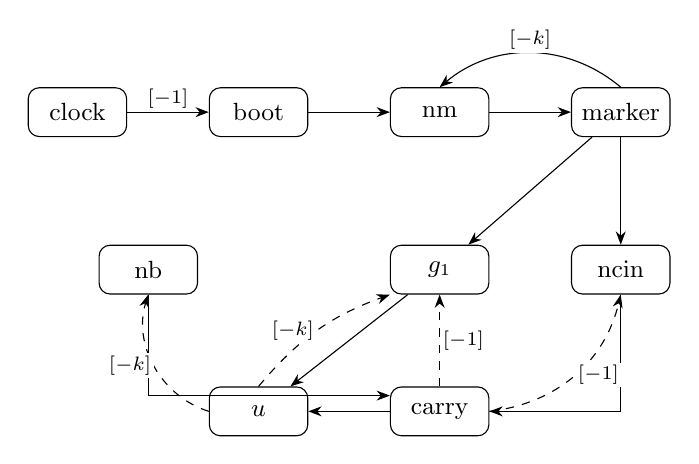
\begin{tikzpicture}[g/.style={draw,rounded corners,minimum width=1.25cm,minimum height=0.62cm,font=\small,fill=white},
  >=Stealth, lab/.style={font=\scriptsize,fill=white,inner sep=1pt}]
\node[g] (clk) at (0,0) {clock};
\node[g] (boot) at (2.3,0) {boot};
\node[g] (nm) at (4.6,0) {nm};
\node[g] (mk) at (6.9,0) {marker};
\node[g] (nb) at (0.9,-2) {nb};
\node[g] (g1) at (4.6,-2) {$g_1$};
\node[g] (ncin) at (6.9,-2) {ncin};
\node[g] (carry) at (4.6,-3.8) {carry};
\node[g] (u) at (2.3,-3.8) {$u$};
\draw[->] (clk) -- node[lab,above]{$[-1]$} (boot);
\draw[->] (boot) -- (nm);
\draw[->] (nm) -- (mk);
\draw[->] (mk.north) to[bend right=40] node[lab,above]{$[-k]$} (nm.north);
\draw[->] (mk) -- (ncin);
\draw[->] (mk) -- (g1);
\draw[->] (ncin) |- (carry);
\draw[->] (nb) |- ([yshift=2mm]carry.west);
\draw[->] (g1) -- (u);
\draw[->] (carry) -- (u);
\draw[->,dashed] (carry.east) to[bend right=35] node[lab,right]{$[-1]$} (ncin.south);
\draw[->,dashed] (carry.north) -- node[lab,right]{$[-1]$} (g1.south);
\draw[->,dashed] (u.west) to[bend left=45] node[lab,left]{$[-k]$} (nb.south);
\draw[->,dashed] (u.north) to[bend left=15] node[lab,left]{$[-k]$} (g1.south west);
\end{tikzpicture}
\caption{The NOR circuit of the bit-serial counter.  Solid edges have delay $0$ (same block);
dashed edges read an earlier block ($[-1]$: previous block, $[-k]$: the same bit of the previous
word).}
\label{fig:circuit}
\end{figure}

\begin{lemma}\label{lem:closed}
Let $\low(w,i)=[\,w\bmod 2^i=2^i-1\,]$ (the lowest $i$ bits of $w$ are all $1$) and let
$\mathrm{bit}_i(x)$ denote bit $i$ of $x$.  The unique solution of the NOR equations is
\begin{align*}
\mathrm{boot}(\tau)&=[\tau=0], & \mathrm{marker}(\tau)&=[k\mid\tau], & \mathrm{nm}&=\neg\mathrm{marker},\\
\mathrm{ncin}(\tau)&=\neg\low(w,i), & \mathrm{nb}(\tau)&=\neg\mathrm{bit}_i(w), &
g_1(\tau)&=\neg(\mathrm{bit}_i(w)\vee\low(w,i)),\\
\mathrm{carry}(\tau)&=\low(w,i+1), & u(\tau)&=\mathrm{bit}_i(w+1).
\end{align*}
In words: word $w$ (blocks $wk,\dots,wk+k-1$) holds the number $(w+1)\bmod 2^k$ in binary, least
significant bit first.
\end{lemma}

\begin{proof}
Each equation is checked directly.  The two arithmetic facts needed are the carry rule
$\low(w,i+1)=\mathrm{bit}_i(w)\wedge\low(w,i)$ and the increment rule
$\mathrm{bit}_i(w+1)=\mathrm{bit}_i(w)\oplus\low(w,i)$; for $u[-k]$ one uses that block $\tau-k$
belongs to word $w-1$, whose value is $w$.  The carry into bit $i$ is
$\mathrm{carry}[-1]\vee\mathrm{marker}=\low(w,i)$.  Uniqueness is immediate by induction on $\tau$.
\end{proof}


\section{The concrete design}\label{sec:design}

A design implementing the counter with $B=260$, $\nclocks$ clocks and $\nmoves$ taps was found by
computer search (Section~\ref{sec:search}):
\begin{center}\small
\begin{tabular}{ll}
\toprule
clocks $C$ & $0,2,3,4,5,6,7,8,25,27,28,29,30,31,32,33,50,60,62,64,65,67,68,123,$\\
 & $225,228,229,230,232$\\
wires $\rho$ & boot $1$, nm $10$, marker $26$, ncin $35$, nb $70$, $g_1$ $98$, carry $147$, $u$ $222$\\
\bottomrule
\end{tabular}
\end{center}
With $K=k-1$ the move set is $S_k=\{(aK+b)\cdot 260+\delta\}$ over the $\nmoves$ taps; explicitly
\begin{multline*}
S_k=\{9,11,13,16,51,72,75,77,84,89,104,110,112,124,135,148,\\
156,171,176,186,209,211,249\}\ \cup\ \{260(k-1)+108,\ 260(k-1)+136,\ 260(k-1)+244\}.
\end{multline*}
The $23$ fixed moves are at most $249<260+108$, so the three $k$-dependent moves (the long delays
feeding nm, nb and $g_1$) are distinct from them and $|S_k|=\nmoves$ for all $k\ge2$, with
$\max S_k=260(k-1)+244=260k-16$.  (In fact the $\nmoves$ residues $\delta$ are distinct, so the moves are
distinct for every $k$.)  Conditions \ref{c:K}--\ref{c:Z0} are finite and are verified mechanically.
Figure~\ref{fig:bitmap} shows the resulting P-positions for $k=3$.

\begin{figure}[t]
\centering
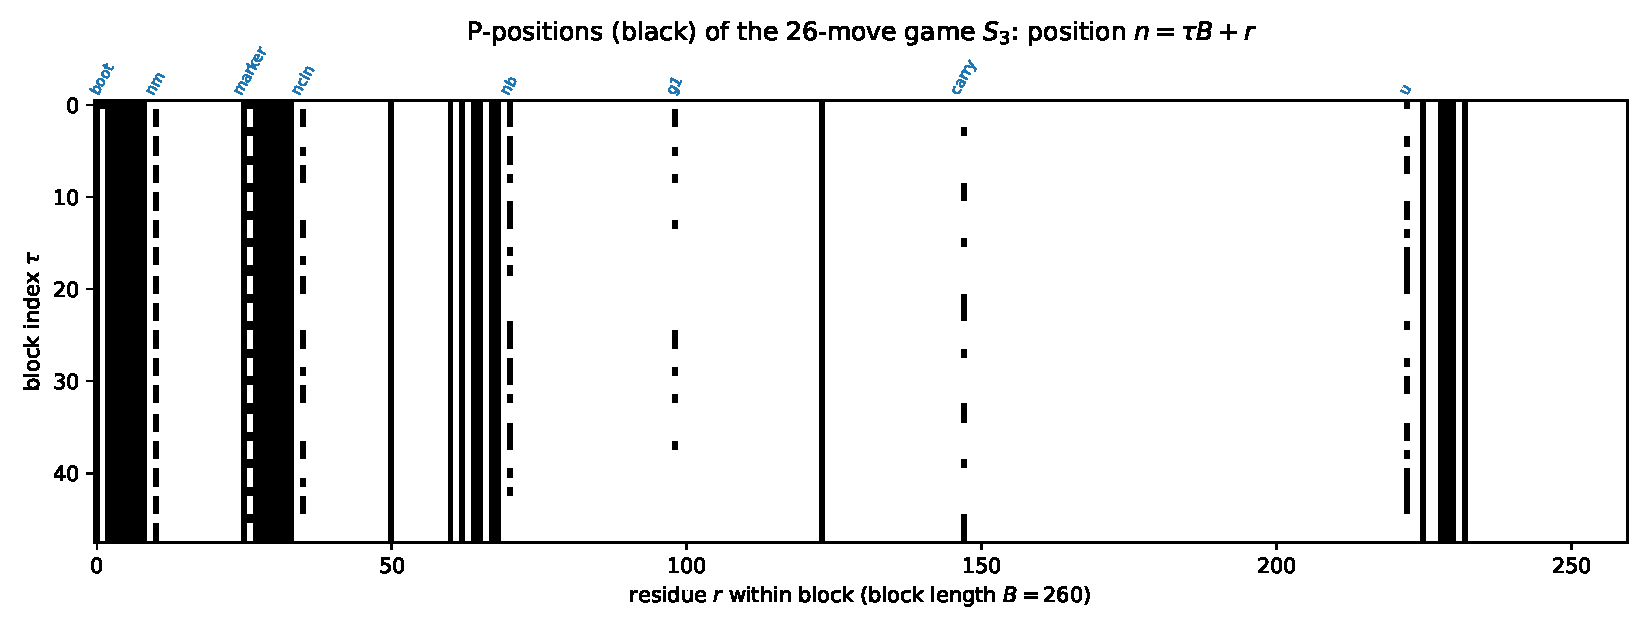
\includegraphics[width=\textwidth]{figs/bitmap.pdf}\\[2mm]
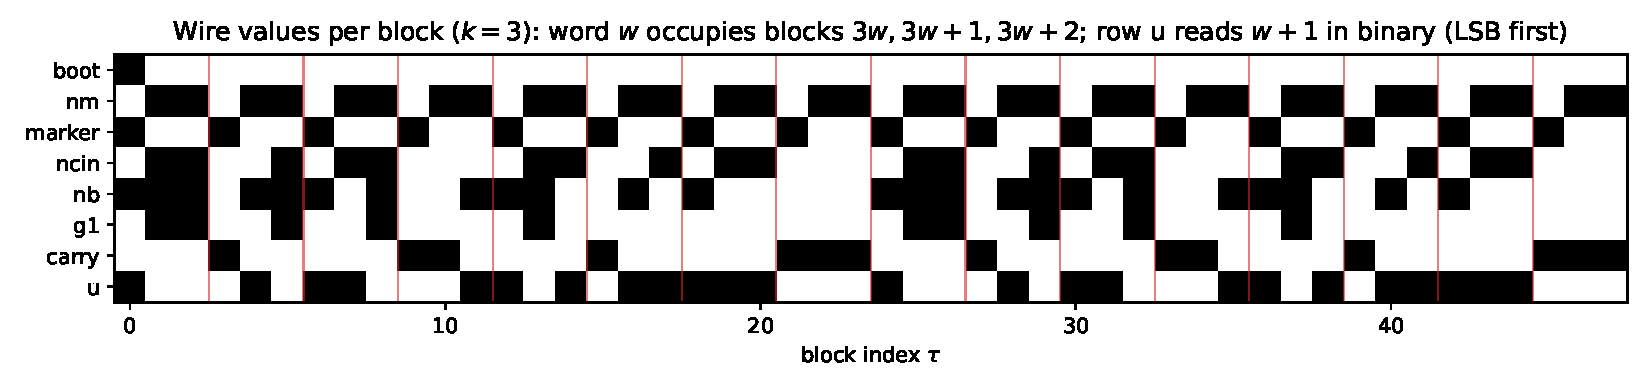
\includegraphics[width=\textwidth]{figs/wires.pdf}
\caption{Top: P-positions of the $\nmoves$-move game $S_3$, one block of $260$ positions per row.  Clocks
are the solid columns; the dashed columns are the eight wires.  Bottom: the wire values; the $u$ row
spells $1,2,3,\dots,7,0,1,\dots$ in binary, three blocks per word.  The period is
$260\cdot 3\cdot 2^3=6240$.}
\label{fig:bitmap}
\end{figure}


\section{The least period}

\begin{theorem}\label{thm:period}
For $k\ge2$ the outcome sequence of $S_k$ satisfies $w(n+P)=w(n)$ for all $n\ge B$, where
$P=B\,k\,2^k$, and every eventual period of $w$ is a multiple of $P$.
\end{theorem}

\begin{proof}
Periodicity follows from Theorem~\ref{thm:sim} and Lemma~\ref{lem:closed}: all closed forms depend
only on $\tau\bmod k$ and $(\tau\div k)\bmod 2^k$ except $\mathrm{boot}$, which is constant for
$\tau\ge1$.  Conversely let $p$ be an eventual period.
(1) If $B\nmid p$, then (a finite check) some clock $c$ is shifted by $p\bmod B$ onto a zero residue,
so $w(\tau B+c)=1\neq 0=w(\tau B+c+p)$ for large $\tau$; hence $p=Bm$.
(2) The marker wire gives $[k\mid \tau+m]=[k\mid\tau]$ for all large $\tau$, hence $k\mid m$, say
$m=km'$.
(3) The $u$ wire gives $\mathrm{bit}_i(w+m'+1)=\mathrm{bit}_i(w+1)$ for all $i<k$ and large $w$,
hence $2^k\mid m'$.  Thus $P\mid p$.
\end{proof}

Theorem~\ref{thm:main} follows, since $\max S_k=260k-16$, and Corollary~\ref{cor:guy} follows because
$2^k$ eventually exceeds $C(260k)^d$.


\section{How the design was found}\label{sec:search}

\begin{enumerate}[leftmargin=*]
\item \textbf{Exploration.}  A C program computes outcome periods by cycle detection on the
$m$-bit shift-register state.  Record periods of max-symmetric five-move sets grow roughly like
$2^{0.33m}$ (confirming Flammenkamp), but along every structured one-parameter family we tried the
periods were erratic---chaotic dynamics that resist proof.  This motivated \emph{designing} rather
than \emph{finding} long periods.
\item \textbf{Layouts.}  Random layouts almost never work: small differences between residues
collide.  Placing wires on a coarse grid $G\cdot Y$ with $Y$ a Sidon set, and clocks in a few
residue classes modulo $G$ chosen so that their sums and differences avoid each other, produced the
first valid design ($B=1157$, $1061$ moves), confirmed by direct simulation for $k\le 8$.
\item \textbf{Heuristic optimisation.}  Choosing covering taps by greedy set cover and running
simulated annealing over wire positions, clock sets and $B$ reduced the number of moves
$1061\to169\to 67\to 56\to 54$.
\item \textbf{Exact optimisation.}  For fixed wire positions, conditions \ref{c:K}--\ref{c:Z0} are
a Boolean constraint problem in the clock indicators $c_r$ and tap indicators $t_\delta$:
``clock sees clock'' is the clause $\neg c_r\vee\neg t_\delta\vee\neg c_{r-\delta}$, a zero residue $r$
needs $c_r\vee\bigvee_\delta(t_\delta\wedge c_{r-\delta})$, and so on.  Minimising $\sum t_\delta$ with the
CP-SAT solver (OR-Tools) found designs with $48$ and then $38$ moves for the annealed wire placement
(the solver's lower bound for that placement is $24$).
\item \textbf{Large-neighbourhood search.}  Letting every wire move within $\pm5$ residues of its current
position (one Boolean per candidate position, with the pairwise difference constraints written out)
and re-solving gave a design with $29$ moves at $B=377$.  It uses many more clocks ($31$ instead of
$17$), grouped in short runs such as $0$--$3$ and $10$--$13$, so that each covering move serves several
zero residues at once, and it leaves every residue above $219$ empty.
\item \textbf{Shorter blocks.}  Re-solving the same model for smaller block lengths, first with the
wires fixed and then again with the wires free inside their windows, gave the final design: $B=260$
and $\nmoves$ moves, better in both respects.
\end{enumerate}
Every candidate was checked by an exact verifier of conditions \ref{c:K}--\ref{c:Z0}, and the final
design by simulating the game itself: for $k=2,\dots,6$ the simulated P-positions coincide with the
counter pattern and the least periods are $2080,6240,16640,41600,99840$.  The number of moves and the growth rate can be traded against each other; the designs we found
(each checked exactly and by simulating the game for $k\le5$) are
\begin{center}\small
\begin{tabular}{cccc}
\toprule
block length $B$ & moves & period & growth \\
\midrule
$377$ & $29$ & $377\,k\,2^k$ & $2^{\max S/377}$ \\
$260$ & $\nmoves$ & $260\,k\,2^k$ & $2^{\max S/260}$ \\
$240$ & $28$ & $240\,k\,2^k$ & $2^{\max S/240}$ \\
\bottomrule
\end{tabular}
\end{center}
The design with $B=260$ is the one formalised; since \texttt{Design.lean} is generated automatically
from a design file, the others can be checked in Lean in the same way.

\section{Formal verification in Lean}\label{sec:lean}

The development (about $3800$ lines, Lean 4.33.1, Mathlib) consists of:
\begin{center}\small
\begin{tabular}{ll}
\toprule
\texttt{Basic.lean} & P-set characterisation, uniqueness, computable \texttt{outcome}\\
\texttt{Arith.lean} & block arithmetic (Lemma~\ref{lem:arith})\\
\texttt{Simulation.lean} & designs, conditions \ref{c:K}--\ref{c:Z0}, Theorem~\ref{thm:sim}\\
\texttt{Bits.lean}, \texttt{Counter.lean} & carry/increment rules, Lemma~\ref{lem:closed}\\
\texttt{Design.lean} & the concrete design; all finite conditions by \texttt{decide +kernel}\\
\texttt{Period.lean} & Theorem~\ref{thm:period}\\
\texttt{Main.lean}, \texttt{Grundy.lean} & Theorem~\ref{thm:main}, Corollary~\ref{cor:guy}, nim-values\\
\texttt{Tests.lean}, \texttt{Exact.lean} & sanity checks; exact size and largest move, $k=6719$\\
\texttt{Layout.lean} & General Layout Lemma (Lemma~\ref{lem:gll}), \texttt{GLL.simulate}\\
\texttt{Transport.lean} & the layout lemma for arbitrary finite types of wire names\\
\texttt{UnivCore.lean} & cellular automata, the universal circuit $U_F$, its NOR equations\\
\texttt{Universal.lean} & order and Sidon placement of the wires; Theorem~\ref{thm:univ}\\
\texttt{TuringSim.lean} & Turing machines, their cellular automata, Corollary~\ref{cor:tm}\\
\texttt{OpenProblem.lean} & Guy's bound for $n$ moves, all $n\ge26$, Open Problem~\ref{op:gap}\\
\bottomrule
\end{tabular}
\end{center}
The game semantics are defined independently of the construction: \texttt{outcome L n} is defined by
well-founded recursion as ``no legal move leads to a position with \texttt{outcome = true}'', and
\texttt{grundy L n} as the minimum excludant of the options' values.  The file \texttt{Design.lean} is
generated from the design found by the search, and the kernel checks conditions
\ref{c:K}--\ref{c:Z0} for it.  No \texttt{sorry}, \texttt{native\_decide} or additional axioms are used.


\section{Universality}\label{sec:pspace}


\subsection{The General Layout Lemma}


The counter was laid out by computer search, but a layout exists for \emph{every} NOR circuit.

\begin{definition}[Circuit]\label{def:circuit}
A \emph{circuit} has wires $0,1,\dots,W-1$; every wire $j$ has a finite list $\mathrm{In}(j)$ of inputs
$(\sigma,d)$, where $\sigma$ is a wire or \textsc{clk} and $d=aK+b$ is a delay.  We require:
(i) $\mathrm{In}(0)=\{(\textsc{clk},1)\}$ (wire $0$ is \emph{boot});
(ii) inputs with delay $0$ come from wires of smaller index;
(iii) no wire is its own input;
(iv) if $\sigma>j$ then $b\ge1$.
\end{definition}

Condition (iii) is necessary: a move that is a multiple of $B$ makes \emph{every} residue read
itself, in particular every clock.

\begin{lemma}[General Layout Lemma]\label{lem:gll}
Let $Y=\{0=y_0<y_1<\dots<y_{W-1}\}$ be a Sidon set (all differences $y_i-y_j$, $i\ne j$, distinct)
with $y_1\ge 2$, let $B'\ge 3y_{W-1}+3$ and $B=13B'$.  Place wire $j$ at residue $13y_j$ and clocks at
$C=\{1,5,12\}$; realise every input $(\sigma,d)$ of wire $j$ by the move $dB+13y_j-\rho(\sigma)$
(where $\rho(\textsc{clk})=5$; for backward edges this is $(d-1)B+(B+13y_j-\rho(\sigma))$), and cover
the zero residues by the rule of Table~\ref{tab:cover}.  Then conditions \ref{c:K}--\ref{c:Z0} hold for
every circuit, so by Theorem~\ref{thm:sim} the subtraction game simulates the circuit.  The design has
$B=O(W^2)$ and at most $B+2+\sum_j|\mathrm{In}(j)|$ moves.
\end{lemma}

\begin{table}[t]
\centering\small
\begin{tabular}{ll}
\toprule
residue $r=13z+\rho$, $z\ge1$ & covering clock $c$ (move $r-c$)\\
\midrule
$\rho\in\{0,1,2,9\}$ & $c=5$\\
$\rho\in\{4,5,8,11,12\}$ & $c=1$\\
$\rho\in\{3,7,10\}$ & $c=1$, except $c=5,12,12$ respectively when $z=B'-1$\\
$\rho=6$ & $c=12$, except $c=1$ when $z=1$\\
\midrule
residue $r<13$ & moves\\
\midrule
$r=3,4$ & $r-1$ \qquad $r=7,8,11$: $r-5$ \qquad $r=9,10$: $r-1$\\
$r=2$ & $B-3$ (clock $5$ of the previous block) and $2$ (boot, block $0$)\\
$r=6$ & $B-6$ (clock $12$ of the previous block) and $6$ (boot, block $0$)\\
\bottomrule
\end{tabular}
\caption{Covering the zero residues in the General Layout Lemma.}
\label{tab:cover}
\end{table}

\begin{proof}
Write residues as $13z+\rho$ with \emph{class} $\rho\in[0,13)$ and \emph{coarse index} $z\in[0,B')$.
Let $X$ be the set of wire and clock residues.  A direct computation gives the classes of the
differences $X-X \pmod B$, as coarse sets modulo $B'$:
\[
\begin{array}{c|ccccccccc}
\text{class} & 0 & 1 & 5 & 8 & 12 & 4,7,11 & 2,6,9 & 3,10\\\hline
\text{coarse} & Y-Y & (Y-1)\cup(-Y) & -Y & Y-1 & (Y-1)\cup(-Y) & \{0\} & \{-1\} & \emptyset
\end{array}
\]
(for instance class $8$ consists of $13y-5$, wire minus clock $5$, with coarse index $y-1$).
Since $Y\subset[0,B'/3)$, these coarse sets do not wrap around.

\emph{Intended moves.}  A wire--wire move has residue $13(y_j-y_i)$.  Applied at a clock it lands in
the clock's class with nonzero coarse index, i.e.\ on a zero residue.  Applied at wire $m$ it lands on
a wire only if $y_m-y_j+y_i\in Y$; as $Y\subset[0,B'/3)$ this is an equality of integers
$y_m+y_i=y_j+y_l$, so the Sidon property forces $m=j$ (the intended target), because $i\ne j$ by
(iii).  A clock move has residue $13y_j-5$ (class $8$); applied at wire $m$ it lands in class $5$ with
coarse index $y_m-y_j$, a clock only if $m=j$; applied at a clock $c$ it lands in class
$c+5\in\{6,10,4\}$, which contains no element of $X$.  Hence \ref{c:W} and \ref{c:W2} hold.

\emph{Covering moves.}  For $z\ge1$ every clock lies below $r$, and the move $r-c$ has class
$\rho-c$ (coarse index $z$) or $\rho-c+13$ (coarse index $z-1$).  Reading off the table of $X-X$, the
choices in Table~\ref{tab:cover} are never differences of two elements of $X$: e.g.\ for $\rho=0$,
$c=5$ gives class $8$ with coarse index $z-1$, which is bad only if $z\in Y$, impossible for a zero
residue of class $0$; for $\rho=3$, $c=1$ gives class $2$, bad only if $z=B'-1$, and then $c=5$ gives
class $11$ with coarse index $B'-2\ne0$.  The remaining cases are identical in nature and use only
$1\notin Y$, $B'-1\notin Y$ and $Y\cap(B'-Y)=\emptyset$.  The residues below $13$ are checked
directly.  Since no covering move is a difference of two elements of $X$, covering moves never make a
clock or a wire see anything, which completes \ref{c:K}, and \ref{c:Z1}, \ref{c:Z0} hold by
construction (boot has value $1$ in block $0$).
\end{proof}

Lemma~\ref{lem:gll} is formally verified in Lean (\texttt{Layout.lean}): the proof reduces every
condition to linear arithmetic modulo $13$ with explicit case splits, discharged by \texttt{omega},
plus one application of the Sidon property.  Before formalising it we also checked it
computationally on $1000$ random circuits with up to $40$ wires and random Sidon sets.

\subsection{Universal games with a bounded number of moves}\label{sec:univ}

The General Layout Lemma produces a game whose number of moves grows with the circuit.  To make the
number of moves \emph{independent of the input} we use a single fixed circuit that enumerates all
inputs by itself.  The only thing that changes from instance to instance is the length of the delay
lines, i.e.\ the numerical value of a few moves.

\begin{definition}[Cellular automata]\label{def:ca}
A \emph{$b$-bit cellular automaton} $F=(f,\iota,\beta)$ consists of a local rule
$f:Q^3\to Q$ on $Q=\{0,1\}^b$, an initialisation map $\iota:\{0,1\}^3\to Q$ and a boundary state
$\beta\in Q$.  For a ring length $L\ge1$, a number $X\ge0$ and $\Lambda\le L$, the run
$\Run_F(L,\Lambda,X,T,i)\in Q$ $(T\ge0,\ 0\le i<L)$ is defined by
\[\Run_F(L,\Lambda,X,0,i)=\iota\bigl(v_i,[i=0],[i=L-1]\bigr),\qquad v_i=\begin{cases}\mathrm{bit}_i(X)&i<\Lambda\\0&i\ge\Lambda\end{cases}\]
and $\Run_F(L,\Lambda,X,T+1,i)=f(c_T(i-1),c_T(i),c_T(i+1))$, where $c_T(i)=\Run_F(L,\Lambda,X,T,i)$ and
$c_T(-1)=c_T(L)=\beta$ (null boundary).  We write $\Run_F(L,X,T,i)=\Run_F(L,L,X,T,i)$.
\end{definition}

The initialisation may depend on whether a cell is the first or the last one; this is how a
Turing-machine simulation places its head and end markers.

\begin{theorem}[Universality with a bounded number of moves]\label{thm:univ}
Let $F$ be a $b$-bit cellular automaton.  There are $B\ge1$, residues $\rho_0,\dots,\rho_{b-1}$ and a
finite list of taps $(a_t,c_t,\delta_t)$ $(t=1,\dots,c)$ with $a_t\in\{0,1\}$ such that for every
$K\ge0$, with ring length $L=K+2$ and
\[S_L=\{(a_tK+c_t)B+\delta_t:\ 1\le t\le c\},\]
and for all $j\ge0$, $0\le T<2^{L}$, $0\le i<L$ and $q<b$:
\[
\bigl((j\,2^{L}+T)L+i\bigr)B+\rho_q\in\cP_{S_L}\iff \Run_F\bigl(L,\,j+1,\,T,\,i\bigr)_q=1 .
\]
Thus the one-parameter family $(S_L)$, all of whose members have at most $c$ moves and
$\max S_L=O(L)$, runs $F$ on the ring of length $L$ from the initial configurations
$X=1,2,3,\dots$ in turn, each for $2^L$ steps.  This theorem is formally verified
(\texttt{SubGame.Univ.universal}).
\end{theorem}

\begin{table}[t]
\centering\footnotesize
\begin{tabular}{@{}l@{\ \ }>{\raggedright\arraybackslash}p{10.3cm}@{\ \ }l@{}}
\toprule
group & wires (NOR of the listed inputs; $[-d]$ = delay $d$ blocks) & value\\
\midrule
framing & $\mathrm{boot}=\NOR(\textsc{clk}[-1])$; $\mathrm{nm}=\NOR(\mathrm{boot},\mathrm{mk}[-L])$;
$\mathrm{mk}=\NOR(\mathrm{nm})$ & $\mathrm{mk}=[i=0]$\\
 & $\mathrm{nlc}=\NOR(\mathrm{mk}[-(L-1)])$, $\mathrm{lc}=\NOR(\mathrm{nlc})$ & $\mathrm{lc}=[i=L-1]$\\
timer & the counter of Section~\ref{sec:counter} with register length $L$ (5 wires) & $u_T=\mathrm{bit}_i(t+1)$\\
run start & $\mathrm{novf}=\NOR(\mathrm{boot},\mathrm{tcarry}[-1])$, $\mathrm{inj}=\NOR(\mathrm{nm},\mathrm{novf})$,
$\mathrm{hold}=\NOR(\mathrm{mk},\mathrm{nrs}[-1])$, $\mathrm{nrs}=\NOR(\mathrm{inj},\mathrm{hold})$, $\mathrm{rs}=\NOR(\mathrm{nrs})$ & $\mathrm{rs}=[T=0]$\\
input & a second counter whose carry-in is $\mathrm{inj}$ (8 wires) & $u_X=\mathrm{bit}_i(j+1)$\\
cells & per state bit $q$: literals $s_q[-L]$, $s_q[-(L\pm1)]$, the neighbours masked by $\mathrm{mk},\mathrm{lc}$
(boundary $\beta$) (9 wires); one NOR per neighbourhood pattern (minterm); $\mathrm{nF}_q=\NOR(\text{minterms
with } f_q=1)$; $t_q=\NOR(\mathrm{rs},\mathrm{nF}_q)$; eight initialisation terms; $\mathrm{ns}_q$; $s_q=\NOR(\mathrm{ns}_q)$ &
$s_q=\Run_F(\dots)_q$\\
\bottomrule
\end{tabular}
\caption{The universal enumerating circuit $U_F$ (one parameter).  Block $\tau=tL+i$ is cell $i$ of
round $t=j2^{L}+T$.  It has $23+21b+2^{3b}$ wires, and its input lists depend on $F$ but not on $L$.}
\label{tab:univ}
\end{table}

\begin{proof}
We build a circuit $U_F$ (Table~\ref{tab:univ}; the complete definition is \texttt{Univ.inp} in
\texttt{UnivCore.lean}, mirrored in \texttt{subgame/univ1.py}) whose delays are $0$, $1$, $L-1$, $L$
and $L+1$, i.e.\ of the form $aK+c$.  Write $\tau=tL+i$ and $t=j2^L+T$.

\emph{Framing.}  As in Lemma~\ref{lem:closed}, $\mathrm{mk}(\tau)=[i=0]$; reading $\mathrm{mk}$ with delay $L-1$
gives $\mathrm{lc}(\tau)=[i=L-1]$.

\emph{Timer.}  The bit-serial counter of Section~\ref{sec:counter} with register length $L$: its bit in
block $\tau$ is $\mathrm{bit}_i(t+1)$ and its carry out of the last cell of round $t$ is
$\low(t,L)=[t\equiv-1\pmod{2^L}]$.

\emph{Run start.}  Hence $\mathrm{novf}$ at cell $0$ is $[T\ne0]$ (at $\tau=0$ it reads $\mathrm{boot}$),
$\mathrm{inj}=[i=0\wedge T=0]$, and the latch $\mathrm{rs}=\mathrm{inj}\vee(\neg\mathrm{mk}\wedge\mathrm{rs}[-1])$ equals
$[T=0]$: runs are the rounds $[j2^L,(j+1)2^L)$.

\emph{Input counter.}  A second counter with carry-in $\mathrm{inj}$ (the carry is cut at $\mathrm{mk}$) is
incremented once per run, during its first round; its bit in block $\tau$ is $\mathrm{bit}_i(j+1)$.

\emph{Cells.}  Let $s_q(\tau)$ be the intended value $\Run_F(L,j+1,T,i)_q$.  For $T\ge1$ the blocks
$\tau-L-1,\tau-L,\tau-L+1$ are cells $i-1,i,i+1$ of round $t-1$, i.e.\ time $T-1$ of the same run; at
$i=0$ (resp.\ $i=L-1$) the left (right) literal is replaced by $\beta$ using $\mathrm{mk}$ ($\mathrm{lc}$).  A
minterm wire is the NOR of the complemented literals, hence is $1$ exactly for its pattern;
$\mathrm{nF}_q=\neg f_q(\text{neighbours})$; and the last NOR levels compute
$s_q=(\neg\mathrm{rs}\wedge f_q)\vee(\mathrm{rs}\wedge\iota_q(u_X,\mathrm{mk},\mathrm{lc}))$.  When $T=0$ the rule
output is ignored, so reads from the previous run (or from negative blocks) do not matter.

The intended values therefore satisfy every NOR equation (this is \texttt{Univ.norEqns}).  Finally we
order the wires so that inputs with delay $0$ come from earlier wires, place wire number $r$ at coarse
position $3^r-1$ (a super-increasing, hence Sidon, sequence), and apply the General Layout Lemma
(transported to arbitrary finite types of wire names); $\rho_q$ is the residue of $s_q$.
\end{proof}

\begin{corollary}[Turing machines, formally verified]\label{cor:tm}
Let $M$ be a deterministic Turing machine with states $Q$, tape alphabet $\Gamma$ and an input map
$\{0,1\}\to\Gamma$, working on the tape cells $0,\dots,L-1$ (a move off the tape leaves the head in
place).  There are $B$, residues $\rho$ and a fixed finite list of taps such that for every $L\ge2$ the
subtraction game $S_L$ with moves $(a_t(L-2)+c_t)B+\delta_t$ satisfies: for every input $X=j+1$ (bit
$i$ on cell $i$), every $T<2^L$ and every cell $i<L$, the positions $((j2^L+T)L+i)B+\rho_x$ that are
P-positions are exactly those whose index $x$ is the content of cell $i$ (symbol, and the state if the head
is there) after $T$ steps of $M$ on input $X$.
\end{corollary}

\begin{proof}
A cell of the automaton holds either a wall (the boundary) or a symbol together with, optionally, the
machine state; the rule moves the head exactly as $M$ does, and keeps it in place when it would move
into a wall.  One step of this automaton is one step of $M$ (\texttt{TM.tmRule\_step}, a case analysis on
the head position relative to the cell).  Encoding the finitely many cell contents one-hot and applying
Theorem~\ref{thm:univ} gives the claim (\texttt{TM.tm\_universal}).
\end{proof}

\paragraph{Two parameters.}  For the binary setting we also need a ring for the tape that is much
longer than the ring carrying the timer and the input.  The same construction with a control ring of
length $L_2$ (timer and input counter) and a tape ring of length $L_1=mL_2$ (the cells), plus a latch
marking the first $L_2$ cells of each tape round and a latch that holds the timer overflow until the
next tape round, gives a family $S_{L_1,L_2}$ with a bounded number of moves and
\[
\bigl((j\,2^{L_2}+T)L_1+i\bigr)B+\rho_q\in\cP_{S_{L_1,L_2}}\iff
\Run_F\bigl(L_1,L_2,\,(j+1)\bmod 2^{L_2},\,T,\,i\bigr)_q=1
\]
for $T<2^{L_2}$ and $i<L_1$: the input occupies the first $L_2$ cells, runs last $2^{L_2}$ tape rounds.
This two-ring circuit ($57$--$59$ wires for $b=1$, \texttt{subgame/univ2.py}) is not formalised; we
checked it as described next.

\paragraph{Validation.}  Both circuits were checked by logic simulation against a direct simulation of
$F$, for all $256$ elementary rules and for random $2$-bit rules with random $\iota$ and $\beta$
($L\in\{3,4,5\}$; $L_1=mL_2$ with $L_2\le4$, $m\le3$), with no mismatch.  We also built the actual
subtraction games and simulated them: for rule $110$ on $L=4$ cells ($123\,181$ moves, $B=124\,917$)
all $2.4\times10^7$ positions of the first three runs agree with the circuit, and for three two-ring
instances ($L_2=3$, $L_1=6$, about $2.6\times10^5$ moves) all positions of four runs agree with the
cellular automaton.

\begin{remark}
The number of moves $c$ is dominated by the covering moves of the General Layout Lemma (about one per
zero residue, i.e.\ about $B$), so it is large; it is nevertheless a constant, independent of $L$ and
of the initial configuration.  For the counter of Section~\ref{sec:counter} exact optimisation reduced
the covering from hundreds of moves to $14$; we have not attempted this for $U_F$.
\end{remark}

\section{Complexity}\label{sec:complexity}

\begin{theorem}[PSPACE-completeness with a bounded number of moves]\label{thm:pspace}
The problem
\begin{center}
\textsc{SubGame}: given a finite set $S\subset\N_{>0}$ in unary and $n\in\N$ in binary, is $n$ a
P-position of the subtraction game $S$?
\end{center}
is PSPACE-complete.  There is a constant $c$ such that it remains PSPACE-complete when restricted to
$|S|\le c$; in fact there is an explicit family $(S_L)_{L\ge3}$ with $|S_L|\le c$ and $\max S_L=O(L)$
such that $\{(1^L,n): n\in\cP_{S_L}\}$ is PSPACE-complete.
\end{theorem}

\begin{proof}
\emph{Membership.}  Compute $w(0),w(1),\dots,w(n)$ keeping only the last $\max S$ values and a
binary counter: space $O(\max S+\log n)$.

\emph{Hardness.}  Let $A$ be a PSPACE-complete language and $M$ a deterministic single-tape machine
deciding it in linear space and time $2^{O(|x|)}$.  Consider the padded language
$A'=\{x10^r: x\in A,\ r\ge0\}$, which is PSPACE-complete as well, and a deterministic machine $M'$
that on an input $y\in\{0,1\}^L$ first locates the last $1$ and then runs $M$ on the prefix before it,
and halts in an absorbing accepting or rejecting state.  It recognises the first and last cell by
marked symbols and never leaves the $L$ cells: choosing $c_1$ large, when the last $1$ of $y$ is at
position $\ell$ it uses at most $c_1(\ell+1)$ cells and at most $2^{c_1(\ell+1)}$ steps.

Let $F$ be the usual cellular automaton simulating $M'$: a cell holds a tape symbol (with the marks
``first'' / ``last''), the machine state if the head is on it, and an \emph{accept flag}; the rule
performs one step of $M'$, and the new flag is the OR of the three old flags and of ``the head is in
the accepting state''.  Let $\iota(v,\textit{first},\textit{last})$ be the cell holding symbol $v$
with the corresponding marks, the head in the initial state iff \textit{first}, and flag $0$; let
$\beta$ be blank.  (Corollary~\ref{cor:tm} is the formal version of this simulation.)  Encode the states
in $b=O(1)$ bits.  Let $(S_L)$ be the one-parameter family of
Theorem~\ref{thm:univ} for $F$; its taps, and hence $c$, depend only on $M$.

Given $x$, let $y=x1$, $L=c_1(|x|+1)+|x|+4$, $X=\sum_i y_i2^i$ (so $1\le X<2^L$), $j=X-1$, $T=2^L-1$ and
$n=\bigl((j2^L+T)L\bigr)B+\rho_{\mathrm{flag}}$.  In run $j$ the automaton starts from $y$ padded by
zeros; $M'$ halts after at most $2^{c_1(|x|+1)}$ steps, and afterwards the flag (if set) spreads one
cell per step, so it reaches cell $0$ before time $2^{c_1(|x|+1)}+L\le 2^L-1$.  By
Theorem~\ref{thm:univ}, $n\in\cP_{S_L}$ iff $x\in A$.  The instance $(S_L,n)$ is computable in
polynomial time: $S_L$ consists of $c$ numbers of size $O(L)$, and $n$ has $O(L)$ bits.
\end{proof}

\begin{theorem}[Binary move sets]\label{thm:exptime}
If the move set $S$ is given in binary (and $n$ in binary), deciding whether $n$ is a P-position of
$S$ is EXPTIME-complete, and it remains EXPTIME-complete when restricted to $|S|\le c$ for a constant
$c$.  Consequently no algorithm with running time polynomial in the input length decides the outcome
of subtraction games with $c$ moves written in binary.
\end{theorem}

\begin{proof}
\emph{Membership.}  The simulation above uses space $O(\max S+\log n)$ and time $O(n|S|)$, both at
most exponential in the input length.

\emph{Hardness.}  Let $M$ decide an EXPTIME-complete language in time $2^{p(|x|)}$ (hence space
$2^{p(|x|)}$) on a one-sided tape; as above let $M'$ run $M$ on the prefix of its input before the last
$1$, and let $F$ simulate $M'$ with a spreading accept flag.  Use the two-parameter family
$S_{L_1,L_2}$ of Section~\ref{sec:univ} (two parameters) with $L_2=p(|x|)+|x|+4$ and $L_1$ the least multiple of $L_2$
exceeding $2^{L_2}$: the input $y=x10\cdots0\in\{0,1\}^{L_2}$ is written on the first $L_2$ of the $L_1$
cells, the machine never reaches the right end of the tape, and it has $2^{L_2}$ steps.  Take
$X=\mathrm{val}(y)$, $j=X-1$, $T=2^{L_2}-1$ and $n=((j2^{L_2}+T)L_1)B+\rho_{\mathrm{flag}}$.  In binary,
$S_{L_1,L_2}$ consists of $c$ numbers of $O(L_2)$ bits and $n$ has $O(L_2)$ bits, so the reduction is
polynomial.  The last statement follows from the time hierarchy theorem
($\mathrm{P}\subsetneq\mathrm{EXPTIME}$).
\end{proof}

Thus the complexity of one-heap subtraction games is governed by the size of the largest move, not
by the number of moves: they are easy for every fixed game, PSPACE-complete for a bounded number of
moves written in unary, and EXPTIME-complete for a bounded number of moves written in binary.

\begin{corollary}[Periods are hard to compute]\label{cor:perhard}
Given $S$ in unary and $p$ in binary, deciding whether the least outcome period of $S$ exceeds $p$
is PSPACE-hard.
\end{corollary}

\begin{proof}
Here a single run suffices.  Let $F$ simulate a linear-space machine $M$ deciding a PSPACE-complete
language, with both halting states absorbing, and encode its states so that the all-zero code
(blank, no head, flag $0$) is quiescent.  Take the circuit of Theorem~\ref{thm:univ} without the timer
and the input counter, and instead OR each state bit $q$ with $\mathrm{OR}_{i\in I_q}\mathrm{boot}[-i]$,
where $I_q$ is the set of cells whose initial state (on input $x$) has bit $q$ equal to $1$; since all
reads in round $0$ return $0$, this loads the initial configuration, at the cost of $O(|x|)$ extra
moves.  After $M$ halts the configuration is frozen, so every wire is periodic with period $L$ blocks.
Add an $L$-bit serial counter as in Section~\ref{sec:counter} whose carry-in is AND-ed with the accept
flag of the current cell.  If $M$ rejects, the counter never moves and the eventual period divides
$BL$; if $M$ accepts, the flag reaches every cell, the counter runs and, as in
Theorem~\ref{thm:period}, the least period is a multiple of $BL2^L$.  Take $p=BL$.
\end{proof}


\section{Discussion and open problems}

A subtraction game is a shift register with a single, fixed nonlinear feedback function, and one
might expect such a rigid object to be computationally weak.  The results above show the opposite:
with a bounded number of moves it can count to $2^{\Omega(\max S)}$, and it can simulate any
space-bounded computation.  Periods are long because the game can compute.

\begin{enumerate}[leftmargin=*]
\item \textbf{How few moves?} (Open Problem~\ref{op:gap})  Our construction needs $\nmoves$ moves;
Flammenkamp's data suggest that five moves may already give exponential periods.  What is the least
$n$ for which periods of $n$-move games are not polynomially bounded?  It lies between $3$ and $26$.  Our search went $1061\to169\to54\to38\to29\to\nmoves$; the
constraint solver's lower bounds for fixed wire placements are far below $\nmoves$, so better
circuits or placements may exist.
\item \textbf{Growth rate.}  Our periods grow like $2^{\max S/260}$ (or $2^{\max S/240}$ with $28$ moves),
much slower than the empirical $2^{0.3\max S}$ of Flammenkamp's records.  Can one prove $2^{c\max S}$ for a larger $c$?  In our
approach $c=1/B$, so the question becomes how short a block can be.
\item \textbf{Complexity threshold.}  Two-move games are easy and games with $c$ moves are
PSPACE-complete.  What is the least number of moves for which \textsc{SubGame} is PSPACE-hard?
\item \textbf{Preperiods.}  The same technique gives exponentially long preperiods (let the counter
halt at its first overflow); it would be interesting to understand the joint behaviour of period and
preperiod for small move sets.
\end{enumerate}

\begin{remark}[Any number of moves $n\ge\nmoves$]\label{rem:pad}
If $\delta$ is a residue that is not a difference of two clock or wire residues (for our design,
e.g.\ $\delta=74$), then from every clock or wire residue a move $\equiv\delta\pmod{260}$ lands on a zero
residue.  Adding moves $qB+\delta$ therefore never creates a
move from a P-position to a P-position, and the P-positions are unchanged.  Hence for every
$n\ge\nmoves$ there are $n$-move games with period $260k2^k$ and largest move $O(k)$.
\end{remark}

\begin{thebibliography}{9}
\bibitem{AB} I.~Althöfer and J.~Bültermann, Superlinear period lengths in some subtraction games,
\emph{Theoret.\ Comput.\ Sci.} 148 (1995) 111--119.
\bibitem{WW} E.~R.~Berlekamp, J.~H.~Conway and R.~K.~Guy, \emph{Winning Ways for Your Mathematical
Plays}, A K Peters, 2001--2004.
\bibitem{Flammenkamp} A.~Flammenkamp, \emph{Lange Perioden in Subtraktions-Spielen}, Dissertation,
Universität Bielefeld, 1997.
\bibitem{LS} U.~Larsson and I.~Saha, A brief conversation about subtraction games,
arXiv:2405.20054 (2024); in \emph{Games of No Chance 6}.
\bibitem{LM} U.~Larsson and H.~Manabe, Additive subtraction games, arXiv:2603.10414 (2026).
\bibitem{LW} U.~Larsson and J.~Wästlund, From heaps of matches to the limits of computability,
\emph{Electron.\ J.\ Combin.} 20 (2013) P41.
\bibitem{DGPS} K.~Burke, A.~Dailly and N.~Oijid, Complexity and algorithms for Arc-Kayles and
Non-Disconnecting Arc-Kayles, arXiv:2404.10390 (2024).
\bibitem{GV} V.~Gurvich and M.~Vyalyi, On computational hardness of multidimensional subtraction
games, \emph{Algorithms} 14 (2021) 71, arXiv:2001.03962.
\bibitem{L12} U.~Larsson, Impartial games emulating one-dimensional cellular automata and
undecidability, arXiv:1201.1039 (2012).
\bibitem{MP} I.~Miklós and L.~Post, Superpolynomial period lengths of the winning positions in the
subtraction game, \emph{Int.\ J.\ Game Theory} (2024), arXiv:2312.02426.
\bibitem{Nowakowski} R.~J.~Nowakowski, Unsolved problems in combinatorial games, in \emph{Games of
No Chance 5}, MSRI Publ.\ 70 (2019) 125--168.
\bibitem{Ward} M.~D.~Ward, A conjecture about periods in subtraction games, arXiv:1606.04029.
\end{thebibliography}

\end{document}
